\section*{Question 6}
\fakesection{6}

We are given the impulse response, $h[n]$, of a low pass FIR filter designed using the Parks-McClellan method. Due to the symmetry of the response, and without loss of generality, we choose to denote the seven values as $h[-3]$ to $h[3]$. The DFT of $h[n]$ is then
\begin{align}
    H(\omega) = \sum_{n=-3}^{3} h[n] e^{-j\omega n}
              = h[0] + \sum_{n=1}^{3} h[n] \left( e^{j\omega n} + e^{-j\omega n} \right)
\end{align}
Applying Euler's formula, (6.1) is equivalent to
\begin{align}
    H(\omega) = h[0] + \sum_{n=1}^{3} h[n] \cdot 2 \cos(\omega n)
\end{align}
The Chebyshev polynomials of the first kind, $T_n$, can be used to relate the multiple-angle cosine functions to powers of a single-angle cosine by $\cos(n\theta)=T_n(\cos\theta)$\footnote{T. J. Rivlin. \textit{Chebyshev Polynomials}, 1st ed. Hoboken, NJ, USA: John Wiley \& Sons, 1974.}. $T_n$ is defined by the recurrence relation\textsuperscript{5}:
\begin{align*}
    T_0(x)     = 1 &&
    T_1(x)     = x &&
    T_{n+1}(x) = 2xT_n(x) - T_{n-1}(x)
\end{align*}
Hence, for the cosine function
\begin{align*}
    T_1(\cos\theta) &= \cos\theta \\
    T_2(\cos\theta) &= 2\cos\theta\cos\theta - 1 = 2\cos^2\theta - 1 \\
    T_3(\cos\theta) &= 2\cos\theta\left( 2\cos^2\theta - 1 \right) - \cos\theta = 4\cos^3\theta - 3\cos\theta
\end{align*}
Thus, we expand (6.2) and apply the Chebyshev polynomials.
\begin{align*}
    H(\omega) &= h[0] + 2 h[1]\cos\omega + 2 h[2]\cos(2\omega) + 2 h[3]\cos(3\omega) \\
              &= h[0] + 2 h[1]\cos\omega + 2 h[2]\left( 2\cos^2\omega - 1 \right) + 2 h[3]\left( 4\cos^3\omega - 3\cos\omega \right) \\
              &= 8 h[3]\cos^3\omega + 4 h[2]\cos^2\omega + 2\left( h[1]\cos\omega - 3h[3]\cos\omega \right) + h[0] - 2 h[2]
\end{align*}
Substituting the given values of $h[n]$, we obtain a polynomial in $\cos\omega$:
\begin{align}
    H(\omega) = -1.0352\cos^3\omega + 0.4804\cos^2\omega + 1.5156\cos\omega + 0.2581
\end{align}
We can express this polynomial in terms of $f=\omega/2\pi$:
\begin{align}
    H(f) = -1.0352\cos^3(2\pi f) + 0.4804\cos^2(2\pi f) + 1.5156\cos(2\pi f) + 0.2581
\end{align}
Or, we can substitute $x=\cos\omega$ to express the result as a polynomial in $x$:
\begin{align}
    H(x) = -1.0352x^3 + 0.4804x^2+ 1.5156x + 0.2581
\end{align}
In this form, it is easier to determine the local extrema, $\frac{dH(\omega)}{d\omega}=0$. Using the chain rule:
\begin{align}
    \frac{dH(\omega)}{d\omega} = \frac{dH(x)}{dx} \cdot \frac{dx(\omega)}{d\omega} = \frac{dH(x)}{dx} \sin\omega = 0
\end{align}
which implies $\frac{dH(x)}{dx}=0$ or $\sin\omega=0$. The derivative of $H(x)$ is trivially found:
\begin{align}
    \frac{dH(x)}{dx} = -3.1056 x^2 + 0.9608 x + 1.5156
\end{align}
and has its roots at $x\approx-0.56082$, 0.87020, or, $\omega=\arccos(x)\approx2.16617$, 0.51520 radians.

\newpage

The other extrema are the roots of $\sin\omega$; we are only interested in those in the range $-\pi<\omega\leq\pi$, which are simply $\omega=0$, $\pi$.

From the roots of $\frac{dH(x)}{dx}$, we can also determine the magnitude of ripple in the pass and stop bands. Since filter is low pass, we infer that $\omega=\omega_{max}\approx0.51520$ is a maximum and $\omega=\omega_{min}\approx2.16617$ is a minimum. The pass and stop band ripple magnitudes, $\delta_p$ and $\delta_s$, respectively, are:
\begin{align*}
    \delta_p = H(\omega_{max}) - 1 \approx 0.25860 &&
    \delta_s = -H(\omega_{min}) \approx 0.25819
\end{align*}
Or, expressed in decibels:
\begin{align*}
    dB(\delta_p) = 20\log\delta_p \approx -11.747 \text{ dB} &&
    dB(\delta_s) = 20\log\delta_s \approx -11.761 \text{ dB}
\end{align*}
In turn, using the pass and stop band ripple magnitudes, we can infer the cutoff and stopband frequencies. These are the frequencies $\omega_c$ and $\omega_s$, respectively, such that
\begin{align*}
    H(\omega_c) = 1 - \delta_p && \text{and} &&
    H(\omega_s) = \delta_s
\end{align*}
Furthermore, both $\omega_c$ and $\omega_s$ necessarily occur between the extrema. Beginning with the cutoff frequency, the mathematics is more easily negotiated in terms of $x_c=\cos\omega_c$ rather than $\omega_c$. That is, we seek $x_c$ such that
\begin{align}
    H(x_c) &= 1 - \delta_p = -1.0352x_c^3 + 0.4804x_c^2+ 1.5156x_c + 0.2581 \\
\intertext{or equivalently,}
         0 &= H(x_c) - (1 - \delta_p) \approx -1.0352x_c^3 + 0.4804x_c^2+ 1.5156x_c - 0.4833
\end{align}
Solving for the roots of (6.8), we obtain three possibilities: $x_c\approx$ -1.15444, 0.30877, 1.30974. However, of these, only the second occurs between the extrema. Thus, the cutoff frequency is
\begin{align*}
    \omega_c = \arccos x_c \approx 1.25690 \text{ (rad)}
\end{align*}
The procedure for the stopband frequency is very similar. We seek $x_s=\cos\omega_s$ such that
\begin{align}
    H(x_s) &= \delta_s = -1.0352x_s^3 + 0.4804x_s^2+ 1.5156x_s + 0.2581 \\
\intertext{or equivalently,}
         0 &= H(x_s) - \delta_s \approx -1.0352x_s^3 + 0.4804x_s^2+ 1.5156x_s - 0.00009
\end{align}
Solving for the roots of (6.10), we obtain three possibilities: $x_s\approx$ -1.00003, 0.00006, 1.46404. Again, of these, only the second occurs between the extrema. Thus, the stopband frequency is
\begin{align*}
    \omega_s = \arccos x_s \approx 1.57074 \text{ (rad)}
\end{align*}
Figure \ref{fig:q6_plot_everything} on the following page plots each of the identified features on top of $H(\omega)$ as a visual confirmation of the correctness of the values.

\newpage

\begin{figure}[ht]
    \centering
    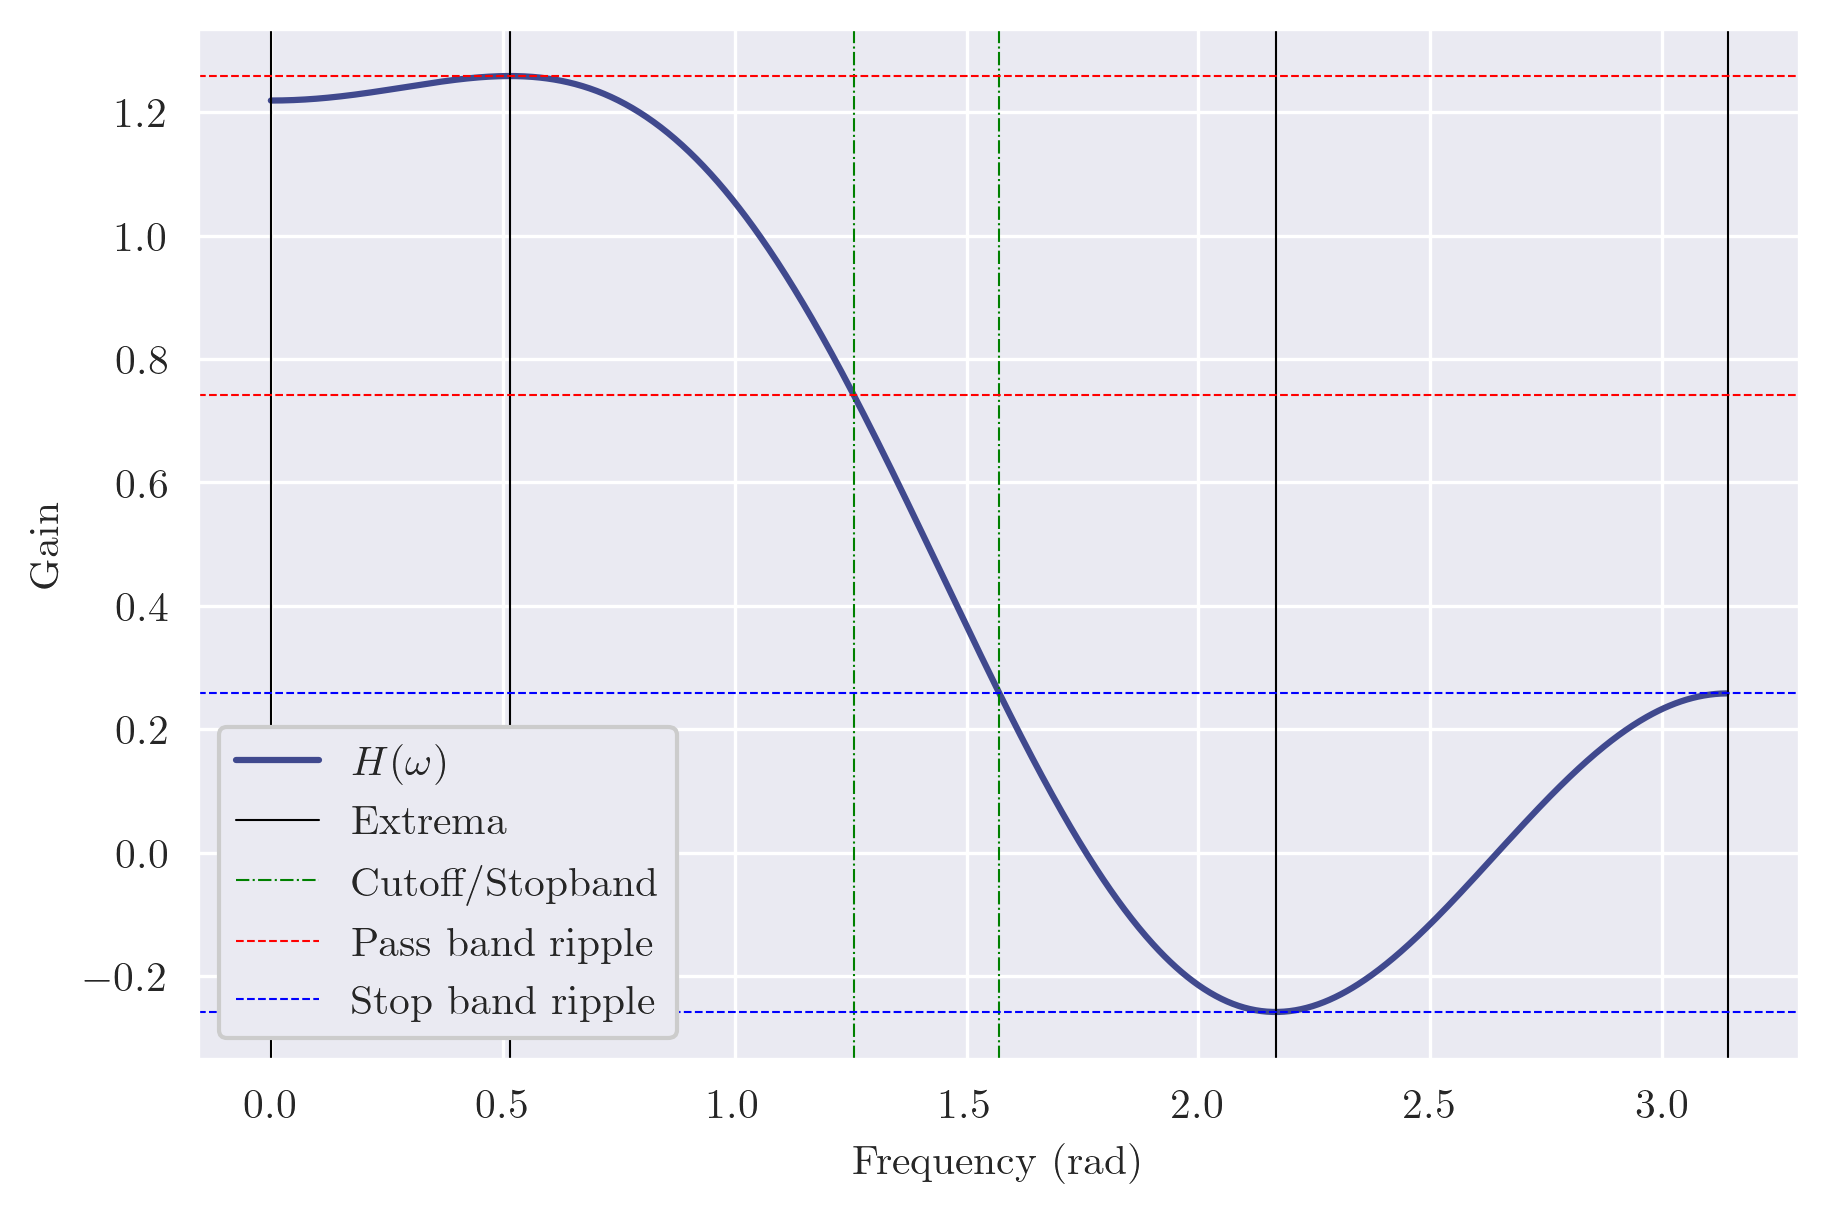
\includegraphics[width=0.95\textwidth]{images/q6_plot_everything.png}
    \caption{All identified extrema, ripple magnitudes, and cutoff and stopband frequencies}
    \label{fig:q6_plot_everything}
\end{figure}

Finally, suppose we were given a polynomial in $x$ and wanted to perform a reverse procedure to obtain an impulse response, $h[n]$. To do so, we would:
\begin{enumerate}
    \item Express the polynomial in terms of $\cos\omega=x$.
    \item Factorise the polynomial to obtain the Chebyshev polynomials of $\cos\omega$.
    \item Convert from exponents $\cos^{n}\omega$ to multiple-angle forms, $\cos(n\omega)$.
    \item Use Euler's formula to express $\cos(n\omega)$ as $(e^{j\omega n} + e^{-j\omega n})/2$.
    \item Determine the values of $h[n]$ from the coefficients of the exponents.
\end{enumerate}
